\section*{Задание}

Реализовать программу по построению графиков функций распределения и функций плотностей для следующих распределений:
\begin{enumerate}
 \item Равномерное распределение
 \item Пуассоновское распределение
 \item Экспоненциальное распределение
 \item Нормальное распределение
 \item K-распределение Эрланга
\end{enumerate}

Для каждого распределения необходимо вычислить и отобразить математическое ожидание и дисперсию.

\newpage

\section*{Теоретическая часть}

\subsection*{1. Равномерное распределение}

Равномерное распределение описывает случайную величину, принимающую значения на отрезке $[a, b]$ с постоянной плотностью вероятности.

\textbf{Функция плотности распределения:}
\begin{equation}
f(x) = 
\begin{cases}
\frac{1}{b - a}, & \text{если } a \leq x \leq b \\
0, & \text{иначе}
\end{cases}
\end{equation}

\textbf{Функция распределения:}
\begin{equation}
F(x) = 
\begin{cases}
0, & \text{если } x < a \\
\frac{x - a}{b - a}, & \text{если } a \leq x \leq b \\
1, & \text{если } x > b
\end{cases}
\end{equation}

\textbf{Математическое ожидание:}
\begin{equation}
E[X] = \frac{a + b}{2}
\end{equation}

\textbf{Дисперсия:}
\begin{equation}
D[X] = \frac{(b - a)^2}{12}
\end{equation}

\subsection*{2. Распределение Пуассона}

Распределение Пуассона описывает вероятность наступления определенного числа событий в фиксированном интервале времени или пространства при известной средней интенсивности $\lambda$.

\textbf{Функция вероятности (для дискретной величины):}
\begin{equation}
P(X = k) = \frac{\lambda^k e^{-\lambda}}{k!}, \quad k = 0, 1, 2, \ldots
\end{equation}

\textbf{Функция распределения:}
\begin{equation}
F(k) = P(X \leq k) = \sum_{i=0}^{\lfloor k \rfloor} \frac{\lambda^i e^{-\lambda}}{i!}
\end{equation}

\textbf{Математическое ожидание:}
\begin{equation}
E[X] = \lambda
\end{equation}

\textbf{Дисперсия:}
\begin{equation}
D[X] = \lambda
\end{equation}

\subsection*{3. Экспоненциальное распределение}

Экспоненциальное распределение описывает время между событиями в процессе Пуассона и характеризуется параметром интенсивности $\lambda$.

\textbf{Функция плотности распределения:}
\begin{equation}
f(x) = 
\begin{cases}
\lambda e^{-\lambda x}, & \text{если } x \geq 0 \\
0, & \text{если } x < 0
\end{cases}
\end{equation}

\textbf{Функция распределения:}
\begin{equation}
F(x) = 
\begin{cases}
1 - e^{-\lambda x}, & \text{если } x \geq 0 \\
0, & \text{если } x < 0
\end{cases}
\end{equation}

\textbf{Математическое ожидание:}
\begin{equation}
E[X] = \frac{1}{\lambda}
\end{equation}

\textbf{Дисперсия:}
\begin{equation}
D[X] = \frac{1}{\lambda^2}
\end{equation}

\subsection*{4. Нормальное распределение}

Нормальное распределение (распределение Гаусса) является одним из наиболее важных распределений в теории вероятностей и описывает множество природных явлений.

\textbf{Функция плотности распределения:}
\begin{equation}
f(x) = \frac{1}{\sigma\sqrt{2\pi}} e^{-\frac{(x - \mu)^2}{2\sigma^2}}
\end{equation}

\textbf{Функция распределения:}
\begin{equation}
F(x) = \frac{1}{2} \left[ 1 + \text{erf}\left( \frac{x - \mu}{\sigma\sqrt{2}} \right) \right]
\end{equation}
где $\text{erf}(z)$ -- функция ошибок:
\begin{equation}
\text{erf}(z) = \frac{2}{\sqrt{\pi}} \int_0^z e^{-t^2} dt
\end{equation}

\textbf{Математическое ожидание:}
\begin{equation}
E[X] = \mu
\end{equation}

\textbf{Дисперсия:}
\begin{equation}
D[X] = \sigma^2
\end{equation}

\subsection*{5. Распределение Эрланга}

Распределение Эрланга является частным случаем гамма-распределения с целым параметром формы $k$ и описывает сумму $k$ независимых экспоненциально распределенных случайных величин.

\textbf{Функция плотности распределения:}
\begin{equation}
f(x) = 
\begin{cases}
\frac{\lambda^k x^{k-1} e^{-\lambda x}}{(k-1)!}, & \text{если } x \geq 0 \\
0, & \text{если } x < 0
\end{cases}
\end{equation}

\textbf{Функция распределения:}
\begin{equation}
F(x) = 
\begin{cases}
1 - \sum_{i=0}^{k-1} \frac{(\lambda x)^i e^{-\lambda x}}{i!}, & \text{если } x \geq 0 \\
0, & \text{если } x < 0
\end{cases}
\end{equation}

\textbf{Математическое ожидание:}
\begin{equation}
E[X] = \frac{k}{\lambda}
\end{equation}

\textbf{Дисперсия:}
\begin{equation}
D[X] = \frac{k}{\lambda^2}
\end{equation}



\section*{Результаты работы программы}

\begin{figure}[H]
\centering
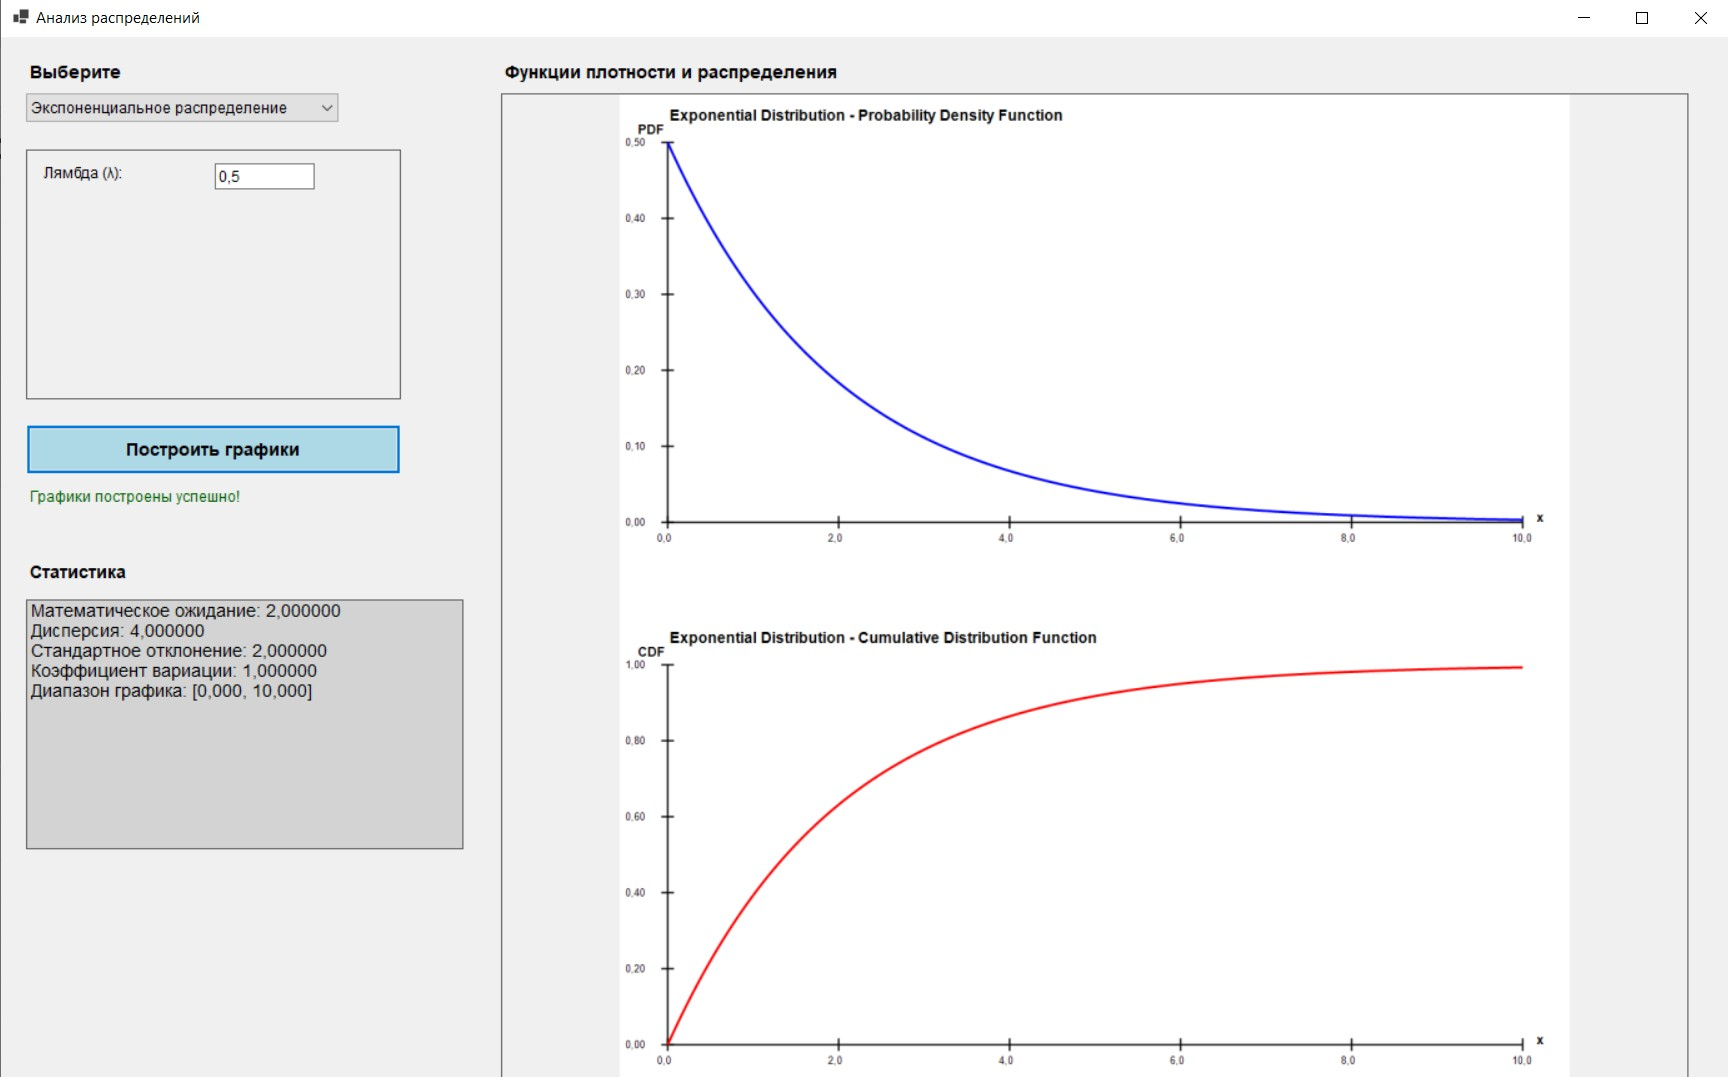
\includegraphics[width=0.9\textwidth]{img/table.jpg}
\caption{Интерфейс программы}
\end{figure}
